% !TeX spellcheck = en_GB

\section{\protect{\emoji{robot}} \texttt{CARSO}: an \textit{introspective artificial neural machine}}{

    \begin{frame}{\protect{\emoji{robot}} Core ideas and intuition (I)}

        Our synthetic \textit{thought process} (\underline{focus on \textit{classification}}):
        \begin{enumerate}
            \item All processing within a (non-stochastic) \textit{NN} is \alert{deterministic} at inference time;
            \item Different outputs from \textit{clean} and successfully \textit{perturbed} inputs must \textit{leave a \alert{different trace}} within the representation of a classifier;
            \item We can use such representation for \textit{adversarial detection}\\ $\rightarrow$ Unsatisfactory!
            \item \textit{And what about \alert{purification}}? We can inform a \textit{\alert{\texttt{cAE}}} with such representation;
        \end{enumerate}

    \begin{block}{Remark!}
    If the purified input is evaluated by the \textit{very same} classifier, the \textit{representation-as-hidden-layers} and the \textit{representation-as-\texttt{cAE}-input} induce \alert{competing} gradients for a \textit{gradient-based} adversary!
    \end{block}
    \end{frame}

    \begin{frame}{\protect{\emoji{robot}} Core ideas and intuition (II)}

    Our synthetic \textit{thought process} (cont.):
    \begin{enumerate}
        \setcounter{enumi}{4}
        \item At inference time, the \alert{representation is more than enough} to reconstruct the input;
        \item We can learn a \texttt{c\alert{V}AE} and sample from the specific purified-input space!
        \item Samples can be later classified and the outputs \alert{aggregated}.
    \end{enumerate}

    \begin{block}{Remark!}
    As a \textit{side effect}, this adds another layer of defence: a \textit{sampling-\alert{invariance}} for the adversary to overcome!
    \end{block}



    \end{frame}

    \begin{frame}{\protect{\emoji{robot}} Another intermezzo: \textit{Conditional Variational Autoencoders}}
        \begin{minipage}[]{0.5\textwidth}
    \vspace{0px}
    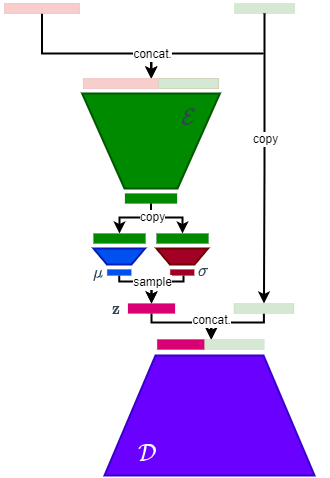
\includegraphics[width=0.91\textwidth, height=0.95\textheight, keepaspectratio]{cvae}
    \end{minipage}
    \begin{minipage}[]{0.45\textwidth}
        \vspace{0pt}
        \textit{Variational Autoencoders} are \textit{artificial neural architectures} able to \alert{sample} from probability densities in the form
        $$ \vec{x} \sim \vec{p}(\vec{\tilde{x}} \condon \phi_1, \dots, \phi_{s\in\mathbb{N}}) \fullstop$$

        They operate in \textit{standard} \alert{autoencoding} settings, with, additionally:
        \begin{itemize}
            \item Code-space sampling;
            \item The approximate \alert{reparametrisation}: $\vec{x} \approx \vec{\tilde{x}} = \netw{D}_{\vec{\theta_{\mathcal{D}}}}(\vec{c} \sim \vec{p}_{\text{latent}}(\vec{c}\condon \netw{E}_{\vec{\theta_{\mathcal{E}}}}(\vec{x})))$
            \item A \textit{loss} constraining the code distribution to a given \alert{structure}: $\mathcal{L}_{\texttt{VAE}} \coloneqq \mathcal{L}_{\text{AE}} + \kldiv(\vec{p}_{\text{latent}},\vec{p}_{\text{lobs}})$
        \end{itemize}

        \textit{Conditional \texttt{VAE}s} extend the sampling to \alert{conditional} distributions of the kind: $${\vec{\tilde{x}_{\text{r.v.}}} \sim \vec{p}(\vec{\tilde{x}_{\text{r.v.}}} \condon \vec{{x}_{\text{c.v.}}}, \phi_1, \dots, \phi_{s\in\mathbb{N}})}$$
    \end{minipage}
    \end{frame}

    \begin{frame}{\protect{\emoji{robot}} Training \texttt{CARSO}}
        \begin{minipage}[]{0.5\textwidth}
            \vspace{0px}
            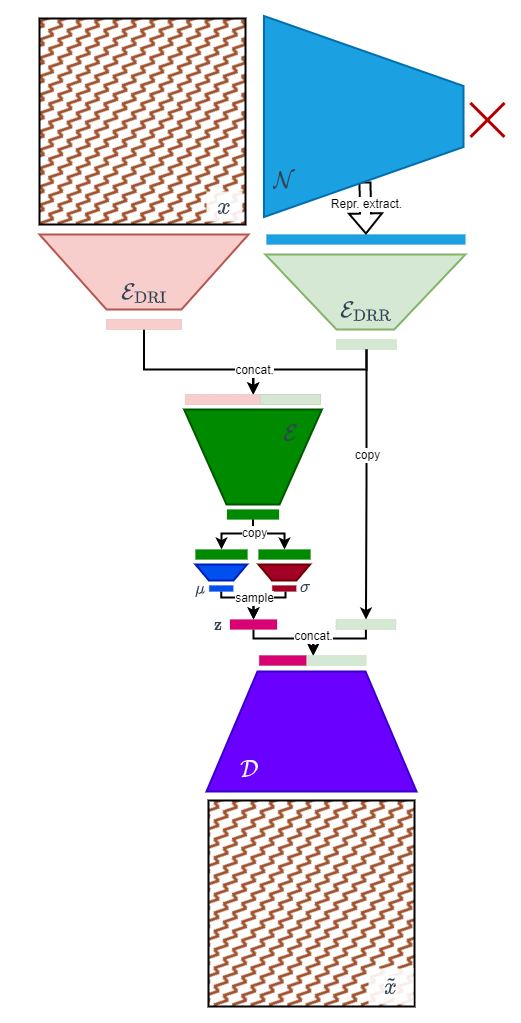
\includegraphics[width=0.91\textwidth, height=0.95\textheight, keepaspectratio]{traindiag}
        \end{minipage}
        \begin{minipage}[]{0.45\textwidth}
            \vspace{0pt}

            \begin{center}
                \underline{\textit{TL;DR:} Just a \textit{fancy \texttt{cVAE}}!}
            \end{center}

            Given an \textit{\alert{adversarially}-pretrained} classifier (for the problem of interest, and according to a given \textit{\alert{threat model}}):
            \hfill\break
            \begin{itemize}
                \item First \textit{classification pass} for representation \alert{extraction};
                \item Pre-encoding and \alert{rebalancing} of input \& representation;
                \item As in \texttt{cVAE}, aiming at \textit{\alert{purified} input} reconstruction from any input.
            \end{itemize}

        \begin{block}{Requirements}
            A dataset of \textit{clean/attacked} inputs to the classifier is needed (but \alert{no labels}!). Threat models may differ.
        \end{block}

        \end{minipage}
    \end{frame}

    \begin{frame}{\protect{\emoji{robot}} Inference with \texttt{CARSO}}
        \begin{minipage}[]{0.5\textwidth}
            \vspace{0px}
            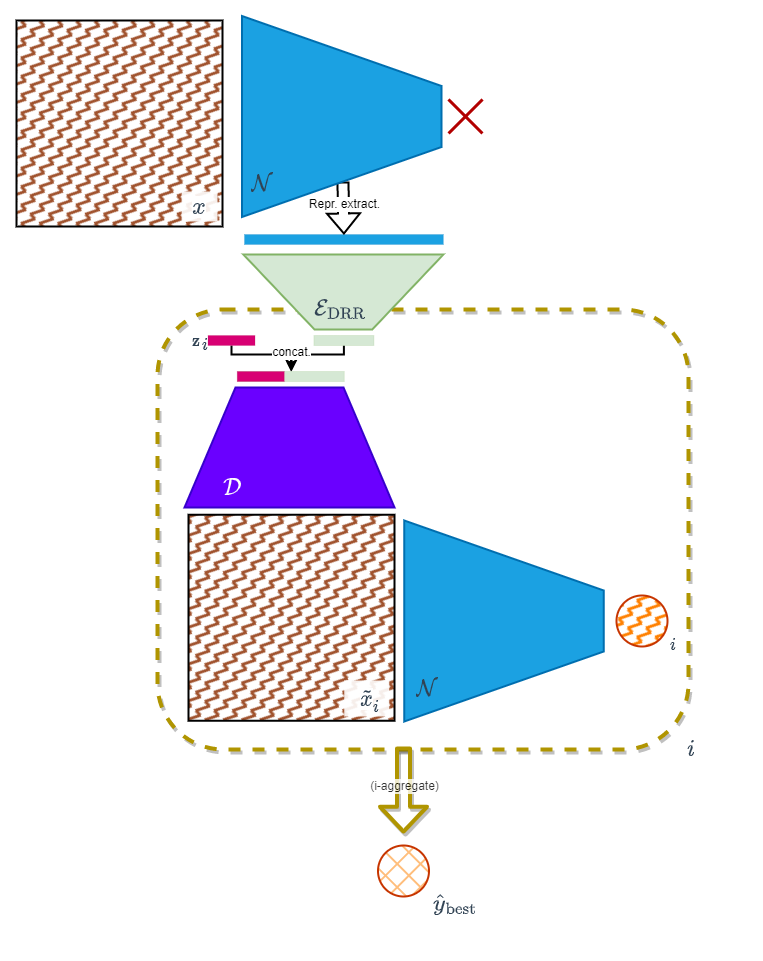
\includegraphics[width=0.95\textwidth, height=0.95\textheight, keepaspectratio]{inferdiag}
        \end{minipage}
        \begin{minipage}[]{0.45\textwidth}
    \vspace{0pt}

    \begin{center}
        \underline{\textit{TL;DR:} Condition, sample, classify, aggregate!}
    \end{center}

    Given the same \textit{adversarially-pretrained} classifier, the just-trained \textit{representation pre-compressor} and \textit{decoder}:
    \hfill\break
    \begin{itemize}
        \item First \textit{classification pass} for representation \alert{extraction};
        \item Representation \textit{pre-encoding};
        \item \alert{Repeated sampling} of \textit{candidate purified inputs};
        \item Second classification pass on such reconstructions, for \alert{actual classification};
        \item \alert{Aggregation} of results.
    \end{itemize}
    \end{minipage}
    \end{frame}

    \begin{frame}{\protect{\emoji{test-tube}} Will it work?}
        \centerline{
    \begin{minipage}[]{0.75\textwidth}
        \begin{quote}{\raggedleft\textsc{M. Budinich} -- \textit{"Introduction to the theory of NNs" course; final remarks before the exam}}
            The difference between a \textit{\alert{great idea}} and an \textit{idea that \alert{works}} is the part in which \alert{you} make it work.\\
            $\textit{ }$
        \end{quote}
    \end{minipage}
    }
    \end{frame}


}
